\documentclass[12pt, oneside, openany]{article}
\usepackage[T1]{fontenc}
\usepackage[spanish, es-tabla, es-lcroman]{babel}
\usepackage[utf8]{inputenc}
\usepackage[document]{ragged2e}
\usepackage{tcolorbox}
\tcbuselibrary{theorems}
\usepackage{cancel}
\usepackage{amssymb}
\usepackage{amsmath}
\usepackage{mathrsfs}
\usepackage{wrapfig}
\usepackage{fancyhdr}
\usepackage{colortbl}
\usepackage{longtable}
\usepackage{graphicx}
\usepackage{subcaption}
\usepackage{xcolor}
\usepackage{tikz}
\usetikzlibrary{positioning}
\usepackage{multicol}
\usepackage{multirow}
\usepackage{lastpage}
\usepackage{pdfpages}
\usepackage{listings}
\usepackage{blindtext}
\spanishdecimal{.}
\usepackage[explicit]{titlesec}
\usepackage[colorlinks=true, linkcolor=black, citecolor=black, urlcolor=blue]{hyperref}
\usepackage[a4paper, total={16cm, 24cm}]{geometry}
\pagestyle{fancy}
\lhead{Muñoz Nuñez Ian Emmanuel}
\rhead{Proyecto 5}
\lfoot{Mtra. María Patricia Ventura Nuñez}
\rfoot{CUCEI}
\renewcommand{\headrulewidth}{1pt}
\renewcommand{\footrulewidth}{1pt}

\setlength{\headheight}{14.49998pt}

\begin{document}
    
    \begin{titlepage}
        \pagenumbering{roman}
        \centering
        {\bfseries\LARGE Universidad de Guadalajara \par}
        \vfill
        {
            \includegraphics[width=0.3\linewidth]{UdG.png}
            \includegraphics[width=0.3\linewidth]{qci.png}
            \par
        }
        \vfill
        {\bfseries\LARGE Seminario de problemas de programación de sistemas reconfigurables \par}
        \vfill
        {\LARGE Diseño de un divisor - Sumador con salida en BCD (display) en un GAL \par}
        \vfill
        {\bfseries\LARGE Nombre: \par}
        \vfill
        {\bfseries\LARGE Muñoz Nuñez Ian Emmanuel \par}
        \vfill
        {\bfseries\LARGE Sección: D01 \par}
        \vfill
        {\bfseries\LARGE Código: 216464457 \par}
        \vfill
        {\bfseries\LARGE Maestra: \par}
        \vfill
        {\bfseries\LARGE María Patricia Ventura Nuñez \par}
        \vfill
        {\bfseries\LARGE Ingeniería robótica \par}
    \end{titlepage}
    
\pagenumbering{arabic}

\newpage
\section{Objetivo}
{\sffamily\large
    \hspace{0.5cm} Solucionar problemas de diseño utilizando las herramientas aprendidas en programación de sistemas reconfigurables.
    
    \hspace{0.5cm} Utilizar hojas de datos de las familias lógicas.
    
    \hspace{0.5cm} Simular circuitos digitales en programas de diseño como \emph{Proteus\texttrademark} e implementarlos físicamente.
    
    \hspace{0.5cm} Diseñar un divisor (ABCD/EF) - Sumador (ABC+DEF) con salida en BCD (display) en un \emph{GAL22v10}.
}

\section{Material}
{\sffamily\large
    \renewcommand{\labelitemi}{$\bullet$}
    \begin{itemize}
        \item Protoboard.
        \item Fuente VCC (5V).
        \item Resistencias de $220\Omega$ y $2k\Omega$.
        \item Dip switch de 8 bits.
        \item 2 GAL22v10.
        \item 2 Display de 7 segmentos.
        \item 2 decodificadores BCD-7 segmentos $\to$ \emph{74LS48}.
    \end{itemize}
}

\newpage
\section{Marco teórico}
\subsection{Tabla de verdad}

{\sffamily

\begin{longtable}[c]{|c||c|c|c|c|c|c|c||c|c|c|c|c|c|c|c|c|}
    \caption{Tabla de verdad. \label{tab:tablaVerdad}} \\
    
    \hline
      & M & A & B & C & D & E & F &  $w_1$ & $x_1$ & $y_1$ & $z_1$ & $.$ & $w_0$ & $x_0$ & $y_0$ & $z_0$ \\
    \hline
    0 & 0 &  0 & 0 & 0 & 0 & 0 & 0 &  1 & 0 & 0 & 0 &  0 &  1 & 0 & 0 & 0 \\
    \hline
    1 & 0 &  0 & 0 & 0 & 0 & 0 & 1 &  0 & 0 & 0 & 0 &  1 &  0 & 0 & 0 & 0 \\
    \hline
    2 & 0 &  0 & 0 & 0 & 0 & 1 & 0 &  0 & 0 & 0 & 0 &  1 &  0 & 0 & 0 & 0 \\
    \hline
    3 & 0 &  0 & 0 & 0 & 0 & 1 & 1 &  0 & 0 & 0 & 0 &  1 &  0 & 0 & 0 & 0 \\
    \hline
    4 & 0 &  0 & 0 & 0 & 1 & 0 & 0 &  1 & 0 & 0 & 0 &  0 &  1 & 0 & 0 & 0 \\
    \hline
    5 & 0 &  0 & 0 & 0 & 1 & 0 & 1 &  0 & 0 & 0 & 1 &  1 &  0 & 0 & 0 & 0 \\
    \hline
    6 & 0 &  0 & 0 & 0 & 1 & 1 & 0 &  0 & 0 & 0 & 0 &  1 &  0 & 1 & 0 & 1 \\
    \hline
    7 & 0 &  0 & 0 & 0 & 1 & 1 & 1 &  0 & 0 & 0 & 0 &  1 &  0 & 0 & 1 & 1 \\
    \hline
    8 & 0 &  0 & 0 & 1 & 0 & 0 & 0 &  1 & 0 & 0 & 0 &  0 &  1 & 0 & 0 & 0 \\
    \hline
    9 & 0 &  0 & 0 & 1 & 0 & 0 & 1 &  0 & 0 & 1 & 0 &  1 &  0 & 0 & 0 & 0 \\
    \hline
    10 & 0 &  0 & 0 & 1 & 0 & 1 & 0 &  0 & 0 & 0 & 1 &  1 &  0 & 0 & 0 & 0 \\
    \hline
    11 & 0 &  0 & 0 & 1 & 0 & 1 & 1 &  0 & 0 & 0 & 0 &  1 &  0 & 1 & 1 & 1 \\
    \hline
    12 & 0 &  0 & 0 & 1 & 1 & 0 & 0 &  1 & 0 & 0 & 0 &  0 &  1 & 0 & 0 & 0 \\
    \hline
    13 & 0 &  0 & 0 & 1 & 1 & 0 & 1 &  0 & 0 & 1 & 1 &  1 &  0 & 0 & 0 & 0 \\
    \hline
    14 & 0 &  0 & 0 & 1 & 1 & 1 & 0 &  0 & 0 & 0 & 1 &  1 &  0 & 1 & 0 & 1 \\
    \hline
    15 & 0 &  0 & 0 & 1 & 1 & 1 & 1 &  0 & 0 & 0 & 1 &  1 &  0 & 0 & 0 & 0 \\
    \hline
    16 & 0 &  0 & 1 & 0 & 0 & 0 & 0 &  1 & 0 & 0 & 0 &  0 &  1 & 0 & 0 & 0 \\
    \hline
    17 & 0 &  0 & 1 & 0 & 0 & 0 & 1 &  0 & 1 & 0 & 0 &  1 &  0 & 0 & 0 & 0 \\
    \hline
    18 & 0 &  0 & 1 & 0 & 0 & 1 & 0 &  0 & 0 & 1 & 0 &  1 &  0 & 0 & 0 & 0 \\
    \hline
    19 & 0 &  0 & 1 & 0 & 0 & 1 & 1 &  0 & 0 & 0 & 1 &  1 &  0 & 0 & 1 & 1 \\
    \hline
    20 & 0 &  0 & 1 & 0 & 1 & 0 & 0 &  1 & 0 & 0 & 0 &  0 &  1 & 0 & 0 & 0 \\
    \hline
    21 & 0 &  0 & 1 & 0 & 1 & 0 & 1 &  0 & 1 & 0 & 1 &  1 &  0 & 0 & 0 & 0 \\
    \hline
    22 & 0 &  0 & 1 & 0 & 1 & 1 & 0 &  0 & 0 & 1 & 0 &  1 &  0 & 1 & 0 & 1 \\
    \hline
    23 & 0 &  0 & 1 & 0 & 1 & 1 & 1 &  0 & 0 & 0 & 1 &  1 &  0 & 1 & 1 & 1 \\
    \hline
    24 & 0 &  0 & 1 & 1 & 0 & 0 & 0 &  1 & 0 & 0 & 0 &  0 &  1 & 0 & 0 & 0 \\
    \hline
    25 & 0 &  0 & 1 & 1 & 0 & 0 & 1 &  0 & 1 & 1 & 0 &  1 &  0 & 0 & 0 & 0 \\
    \hline
    26 & 0 &  0 & 1 & 1 & 0 & 1 & 0 &  0 & 0 & 1 & 1 &  1 &  0 & 0 & 0 & 0 \\
    \hline
    27 & 0 &  0 & 1 & 1 & 0 & 1 & 1 &  0 & 0 & 1 & 0 &  1 &  0 & 0 & 0 & 0 \\
    \hline
    28 & 0 &  0 & 1 & 1 & 1 & 0 & 0 &  1 & 0 & 0 & 0 &  0 &  1 & 0 & 0 & 0 \\
    \hline
    29 & 0 &  0 & 1 & 1 & 1 & 0 & 1 &  0 & 1 & 1 & 1 &  1 &  0 & 0 & 0 & 0 \\
    \hline
    30 & 0 &  0 & 1 & 1 & 1 & 1 & 0 &  0 & 0 & 1 & 1 &  1 &  0 & 1 & 0 & 1 \\
    \hline
    31 & 0 &  0 & 1 & 1 & 1 & 1 & 1 &  0 & 0 & 1 & 0 &  1 &  0 & 0 & 1 & 1 \\
    \hline
    32 & 0 &  1 & 0 & 0 & 0 & 0 & 0 &  1 & 0 & 0 & 0 &  0 &  1 & 0 & 0 & 0 \\
    \hline
    33 & 0 &  1 & 0 & 0 & 0 & 0 & 1 &  1 & 0 & 0 & 0 &  1 &  0 & 0 & 0 & 0 \\
    \hline
    34 & 0 &  1 & 0 & 0 & 0 & 1 & 0 &  0 & 1 & 0 & 0 &  1 &  0 & 0 & 0 & 0 \\
    \hline
    35 & 0 &  1 & 0 & 0 & 0 & 1 & 1 &  0 & 0 & 1 & 0 &  1 &  0 & 1 & 1 & 1 \\
    \hline
    36 & 0 &  1 & 0 & 0 & 1 & 0 & 0 &  1 & 0 & 0 & 0 &  0 &  1 & 0 & 0 & 0 \\
    \hline
    37 & 0 &  1 & 0 & 0 & 1 & 0 & 1 &  1 & 0 & 0 & 1 &  1 &  0 & 0 & 0 & 0 \\
    \hline
    38 & 0 &  1 & 0 & 0 & 1 & 1 & 0 &  0 & 1 & 0 & 0 &  1 &  0 & 1 & 0 & 1 \\
    \hline
    39 & 0 &  1 & 0 & 0 & 1 & 1 & 1 &  0 & 0 & 1 & 1 &  1 &  0 & 0 & 0 & 0 \\
    \hline
    40 & 0 &  1 & 0 & 1 & 0 & 0 & 0 &  1 & 0 & 0 & 0 &  0 &  1 & 0 & 0 & 0 \\
    \hline
    41 & 0 &  1 & 0 & 1 & 0 & 0 & 1 &  0 & 0 & 0 & 1 &  0 &  0 & 0 & 0 & 0 \\
    \hline
    42 & 0 &  1 & 0 & 1 & 0 & 1 & 0 &  0 & 0 & 1 & 1 &  1 &  0 & 0 & 0 & 0 \\
    \hline
    43 & 0 &  1 & 0 & 1 & 0 & 1 & 1 &  0 & 0 & 1 & 1 &  1 &  0 & 0 & 1 & 1 \\
    \hline
    44 & 0 &  1 & 0 & 1 & 1 & 0 & 0 &  1 & 0 & 0 & 0 &  0 &  1 & 0 & 0 & 0 \\
    \hline
    45 & 0 &  1 & 0 & 1 & 1 & 0 & 1 &  0 & 0 & 0 & 1 &  0 &  0 & 0 & 0 & 1 \\
    \hline
    46 & 0 &  1 & 0 & 1 & 1 & 1 & 0 &  0 & 1 & 0 & 1 &  1 &  0 & 1 & 0 & 1 \\
    \hline
    47 & 0 &  1 & 0 & 1 & 1 & 1 & 1 &  0 & 0 & 1 & 1 &  1 &  0 & 1 & 1 & 1 \\
    \hline
    48 & 0 &  1 & 1 & 0 & 0 & 0 & 0 &  1 & 0 & 0 & 0 &  0 &  1 & 0 & 0 & 0 \\
    \hline
    49 & 0 &  1 & 1 & 0 & 0 & 0 & 1 &  0 & 0 & 0 & 1 &  0 &  0 & 0 & 1 & 0 \\
    \hline
    50 & 0 &  1 & 1 & 0 & 0 & 1 & 0 &  0 & 1 & 1 & 0 &  1 &  0 & 0 & 0 & 0 \\
    \hline
    51 & 0 &  1 & 1 & 0 & 0 & 1 & 1 &  0 & 1 & 0 & 0 &  1 &  0 & 0 & 0 & 0 \\
    \hline
    52 & 0 &  1 & 1 & 0 & 1 & 0 & 0 &  1 & 0 & 0 & 0 &  0 &  1 & 0 & 0 & 0 \\
    \hline
    53 & 0 &  1 & 1 & 0 & 1 & 0 & 1 &  0 & 0 & 0 & 1 &  0 &  0 & 0 & 1 & 1 \\
    \hline
    54 & 0 &  1 & 1 & 0 & 1 & 1 & 0 &  0 & 1 & 1 & 0 &  1 &  0 & 1 & 0 & 1 \\
    \hline
    55 & 0 &  1 & 1 & 0 & 1 & 1 & 1 &  0 & 1 & 0 & 0 &  1 &  0 & 0 & 1 & 1 \\
    \hline
    56 & 0 &  1 & 1 & 1 & 0 & 0 & 0 &  1 & 0 & 0 & 0 &  0 &  1 & 0 & 0 & 0 \\
    \hline
    57 & 0 &  1 & 1 & 1 & 0 & 0 & 1 &  0 & 0 & 0 & 1 &  0 &  0 & 1 & 0 & 0 \\
    \hline
    58 & 0 &  1 & 1 & 1 & 0 & 1 & 0 &  0 & 1 & 1 & 1 &  1 &  0 & 0 & 0 & 0 \\
    \hline
    59 & 0 &  1 & 1 & 1 & 0 & 1 & 1 &  0 & 1 & 0 & 0 &  1 &  0 & 1 & 1 & 1 \\
    \hline
    60 & 0 &  1 & 1 & 1 & 1 & 0 & 0 &  1 & 0 & 0 & 0 &  0 &  1 & 0 & 0 & 0 \\
    \hline
    61 & 0 &  1 & 1 & 1 & 1 & 0 & 1 &  0 & 0 & 0 & 1 &  0 &  0 & 1 & 0 & 1 \\
    \hline
    62 & 0 &  1 & 1 & 1 & 1 & 1 & 0 &  0 & 1 & 1 & 1 &  1 &  0 & 1 & 0 & 1 \\
    \hline
    63 & 0 &  1 & 1 & 1 & 1 & 1 & 1 &  0 & 1 & 0 & 1 &  1 &  0 & 0 & 0 & 0 \\
    \hline
    64 & 1 &  0 & 0 & 0 & 0 & 0 & 0 &  0 & 0 & 0 & 0 &  0 &  0 & 0 & 0 & 0 \\
    \hline
    65 & 1 &  0 & 0 & 0 & 0 & 0 & 1 &  0 & 0 & 0 & 0 &  0 &  0 & 0 & 0 & 1 \\
    \hline
    66 & 1 &  0 & 0 & 0 & 0 & 1 & 0 &  0 & 0 & 0 & 0 &  0 &  0 & 0 & 1 & 0 \\
    \hline
    67 & 1 &  0 & 0 & 0 & 0 & 1 & 1 &  0 & 0 & 0 & 0 &  0 &  0 & 0 & 1 & 1 \\
    \hline
    68 & 1 &  0 & 0 & 0 & 1 & 0 & 0 &  0 & 0 & 0 & 0 &  0 &  0 & 1 & 0 & 0 \\
    \hline
    69 & 1 &  0 & 0 & 0 & 1 & 0 & 1 &  0 & 0 & 0 & 0 &  0 &  0 & 1 & 0 & 1 \\
    \hline
    70 & 1 &  0 & 0 & 0 & 1 & 1 & 0 &  0 & 0 & 0 & 0 &  0 &  0 & 1 & 1 & 0 \\
    \hline
    71 & 1 &  0 & 0 & 0 & 1 & 1 & 1 &  0 & 0 & 0 & 0 &  0 &  0 & 1 & 1 & 1 \\
    \hline
    72 & 1 &  0 & 0 & 1 & 0 & 0 & 0 &  0 & 0 & 0 & 0 &  0 &  0 & 0 & 0 & 1 \\
    \hline
    73 & 1 &  0 & 0 & 1 & 0 & 0 & 1 &  0 & 0 & 0 & 0 &  0 &  0 & 0 & 1 & 0 \\
    \hline
    74 & 1 &  0 & 0 & 1 & 0 & 1 & 0 &  0 & 0 & 0 & 0 &  0 &  0 & 0 & 1 & 1 \\
    \hline
    75 & 1 &  0 & 0 & 1 & 0 & 1 & 1 &  0 & 0 & 0 & 0 &  0 &  0 & 1 & 0 & 0 \\
    \hline
    76 & 1 &  0 & 0 & 1 & 1 & 0 & 0 &  0 & 0 & 0 & 0 &  0 &  0 & 1 & 0 & 1 \\
    \hline
    77 & 1 &  0 & 0 & 1 & 1 & 0 & 1 &  0 & 0 & 0 & 0 &  0 &  0 & 1 & 1 & 0 \\
    \hline
    78 & 1 &  0 & 0 & 1 & 1 & 1 & 0 &  0 & 0 & 0 & 0 &  0 &  0 & 1 & 1 & 1 \\
    \hline
    79 & 1 &  0 & 0 & 1 & 1 & 1 & 1 &  0 & 0 & 0 & 0 &  0 &  1 & 0 & 0 & 0 \\
    \hline
    80 & 1 &  0 & 1 & 0 & 0 & 0 & 0 &  0 & 0 & 0 & 0 &  0 &  0 & 0 & 1 & 0 \\
    \hline
    81 & 1 &  0 & 1 & 0 & 0 & 0 & 1 &  0 & 0 & 0 & 0 &  0 &  0 & 0 & 1 & 1 \\
    \hline
    82 & 1 &  0 & 1 & 0 & 0 & 1 & 0 &  0 & 0 & 0 & 0 &  0 &  0 & 1 & 0 & 0 \\
    \hline
    83 & 1 &  0 & 1 & 0 & 0 & 1 & 1 &  0 & 0 & 0 & 0 &  0 &  0 & 1 & 0 & 1 \\
    \hline
    84 & 1 &  0 & 1 & 0 & 1 & 0 & 0 &  0 & 0 & 0 & 0 &  0 &  0 & 1 & 1 & 0 \\
    \hline
    85 & 1 &  0 & 1 & 0 & 1 & 0 & 1 &  0 & 0 & 0 & 0 &  0 &  0 & 1 & 1 & 1 \\
    \hline
    86 & 1 &  0 & 1 & 0 & 1 & 1 & 0 &  0 & 0 & 0 & 0 &  0 &  1 & 0 & 0 & 0 \\
    \hline
    87 & 1 &  0 & 1 & 0 & 1 & 1 & 1 &  0 & 0 & 0 & 0 &  0 &  1 & 0 & 0 & 1 \\
    \hline
    88 & 1 &  0 & 1 & 1 & 0 & 0 & 0 &  0 & 0 & 0 & 0 &  0 &  0 & 0 & 1 & 1 \\
    \hline
    89 & 1 &  0 & 1 & 1 & 0 & 0 & 1 &  0 & 0 & 0 & 0 &  0 &  0 & 1 & 0 & 0 \\
    \hline
    90 & 1 &  0 & 1 & 1 & 0 & 1 & 0 &  0 & 0 & 0 & 0 &  0 &  0 & 1 & 0 & 1 \\
    \hline
    91 & 1 &  0 & 1 & 1 & 0 & 1 & 1 &  0 & 0 & 0 & 0 &  0 &  0 & 1 & 1 & 0 \\
    \hline
    92 & 1 &  0 & 1 & 1 & 1 & 0 & 0 &  0 & 0 & 0 & 0 &  0 &  0 & 1 & 1 & 1 \\
    \hline
    93 & 1 &  0 & 1 & 1 & 1 & 0 & 1 &  0 & 0 & 0 & 0 &  0 &  1 & 0 & 0 & 0 \\
    \hline
    94 & 1 &  0 & 1 & 1 & 1 & 1 & 0 &  0 & 0 & 0 & 0 &  0 &  1 & 0 & 0 & 1 \\
    \hline
    95 & 1 &  0 & 1 & 1 & 1 & 1 & 1 &  0 & 0 & 0 & 1 &  0 &  0 & 0 & 0 & 0 \\
    \hline
    96 & 1 &  1 & 0 & 0 & 0 & 0 & 0 &  0 & 0 & 0 & 0 &  0 &  0 & 1 & 0 & 0 \\
    \hline
    97 & 1 &  1 & 0 & 0 & 0 & 0 & 1 &  0 & 0 & 0 & 0 &  0 &  0 & 1 & 0 & 1 \\
    \hline
    98 & 1 &  1 & 0 & 0 & 0 & 1 & 0 &  0 & 0 & 0 & 0 &  0 &  0 & 1 & 1 & 0 \\
    \hline
    99 & 1 &  1 & 0 & 0 & 0 & 1 & 1 &  0 & 0 & 0 & 0 &  0 &  0 & 1 & 1 & 1 \\
    \hline
    100 & 1 &  1 & 0 & 0 & 1 & 0 & 0 &  0 & 0 & 0 & 0 &  0 &  1 & 0 & 0 & 0 \\
    \hline
    101 & 1 &  1 & 0 & 0 & 1 & 0 & 1 &  0 & 0 & 0 & 0 &  0 &  1 & 0 & 0 & 1 \\
    \hline
    102 & 1 &  1 & 0 & 0 & 1 & 1 & 0 &  0 & 0 & 0 & 1 &  0 &  0 & 0 & 0 & 0 \\
    \hline
    103 & 1 &  1 & 0 & 0 & 1 & 1 & 1 &  0 & 0 & 0 & 1 &  0 &  0 & 0 & 0 & 1 \\
    \hline
    104 & 1 &  1 & 0 & 1 & 0 & 0 & 0 &  0 & 0 & 0 & 0 &  0 &  0 & 1 & 0 & 1 \\
    \hline
    105 & 1 &  1 & 0 & 1 & 0 & 0 & 1 &  0 & 0 & 0 & 0 &  0 &  0 & 1 & 1 & 0 \\
    \hline
    106 & 1 &  1 & 0 & 1 & 0 & 1 & 0 &  0 & 0 & 0 & 0 &  0 &  0 & 1 & 1 & 1 \\
    \hline
    107 & 1 &  1 & 0 & 1 & 0 & 1 & 1 &  0 & 0 & 0 & 0 &  0 &  1 & 0 & 0 & 0 \\
    \hline
    108 & 1 &  1 & 0 & 1 & 1 & 0 & 0 &  0 & 0 & 0 & 0 &  0 &  1 & 0 & 0 & 1 \\
    \hline
    109 & 1 &  1 & 0 & 1 & 1 & 0 & 1 &  0 & 0 & 0 & 1 &  0 &  0 & 0 & 0 & 0 \\
    \hline
    110 & 1 &  1 & 0 & 1 & 1 & 1 & 0 &  0 & 0 & 0 & 1 &  0 &  0 & 0 & 0 & 1 \\
    \hline
    111 & 1 &  1 & 0 & 1 & 1 & 1 & 1 &  0 & 0 & 0 & 1 &  0 &  0 & 0 & 1 & 0 \\
    \hline
    112 & 1 &  1 & 1 & 0 & 0 & 0 & 0 &  0 & 0 & 0 & 0 &  0 &  0 & 1 & 1 & 0 \\
    \hline
    113 & 1 &  1 & 1 & 0 & 0 & 0 & 1 &  0 & 0 & 0 & 0 &  0 &  0 & 1 & 1 & 1 \\
    \hline
    114 & 1 &  1 & 1 & 0 & 0 & 1 & 0 &  0 & 0 & 0 & 0 &  0 &  1 & 0 & 0 & 0 \\
    \hline
    115 & 1 &  1 & 1 & 0 & 0 & 1 & 1 &  0 & 0 & 0 & 0 &  0 &  1 & 0 & 0 & 1 \\
    \hline
    116 & 1 &  1 & 1 & 0 & 1 & 0 & 0 &  0 & 0 & 0 & 1 &  0 &  0 & 0 & 0 & 0 \\
    \hline
    117 & 1 &  1 & 1 & 0 & 1 & 0 & 1 &  0 & 0 & 0 & 1 &  0 &  0 & 0 & 0 & 1 \\
    \hline
    118 & 1 &  1 & 1 & 0 & 1 & 1 & 0 &  0 & 0 & 0 & 1 &  0 &  0 & 0 & 1 & 0 \\
    \hline
    119 & 1 &  1 & 1 & 0 & 1 & 1 & 1 &  0 & 0 & 0 & 1 &  0 &  0 & 0 & 1 & 1 \\
    \hline
    120 & 1 &  1 & 1 & 1 & 0 & 0 & 0 &  0 & 0 & 0 & 0 &  0 &  0 & 1 & 1 & 1 \\
    \hline
    121 & 1 &  1 & 1 & 1 & 0 & 0 & 1 &  0 & 0 & 0 & 0 &  0 &  1 & 0 & 0 & 0 \\
    \hline
    122 & 1 &  1 & 1 & 1 & 0 & 1 & 0 &  0 & 0 & 0 & 0 &  0 &  1 & 0 & 0 & 1 \\
    \hline
    123 & 1 &  1 & 1 & 1 & 0 & 1 & 1 &  0 & 0 & 0 & 1 &  0 &  0 & 0 & 0 & 0 \\
    \hline
    124 & 1 &  1 & 1 & 1 & 1 & 0 & 0 &  0 & 0 & 0 & 1 &  0 &  0 & 0 & 0 & 1 \\
    \hline
    125 & 1 &  1 & 1 & 1 & 1 & 0 & 1 &  0 & 0 & 0 & 1 &  0 &  0 & 0 & 1 & 0 \\
    \hline
    126 & 1 &  1 & 1 & 1 & 1 & 1 & 0 &  0 & 0 & 0 & 1 &  0 &  0 & 0 & 1 & 1 \\
    \hline
    127 & 1 &  1 & 1 & 1 & 1 & 1 & 1 &  0 & 0 & 0 & 1 &  0 &  0 & 1 & 0 & 0 \\
    \hline
    
\end{longtable}

}

\newpage
\subsection{Ecuaciones lógicas }
{\sffamily
    \begin{equation*}
        w_1 = (\overline{M}\,\overline{E}\,\overline{F}\,) + (\overline{M}\,A\,\overline{B}\,\overline{C}\,\overline{E})
    \end{equation*}
    
    \begin{equation*}
        x_1 = (\overline{M}\,\overline{A}\,B\,\overline{E}\,F) + (\overline{M}\,A\,E\,\overline{F}) + (\overline{M}\,A\,B\,E)
    \end{equation*}
    
    \begin{equation*}
        y_1 = (\overline{M}\,\overline{A}\,C\,\overline{E}\,F) + (\overline{M}\,B\,E\,\overline{F}) + (\overline{M}\,A\,\overline{B}\,E\,F) + (\overline{M}\,\overline{A}\,B\,C\,E)
    \end{equation*}
    
    \begin{multline*}
        z_1 = (MBCDEF) + (MADE) + (MABD) + (MABCEF) + (\overline{M}\,C\,E\,\overline{F}) \\
        + (\overline{M}\,D\,\overline{E}\,F) + (\overline{M}\,\overline{A}\,B\,\overline{C}\,E\,F) + (ACDF) + (\overline{M}\,A\,B\,\overline{E}\,F) + (\overline{M}\,\overline{B}\,C\,D\,E) \\
        + (\overline{M}\,A\,\overline{B}\,D\,F) + (\overline{M}\,A\,\overline{B}\,C\,F)
    \end{multline*}
    
    \begin{equation*}
        P = (\overline{M}\,\overline{B}\,\overline{C}\,F) + (\overline{M}\,\overline{A}\,F) + (\overline{M}\,E)
    \end{equation*}
    
    \begin{multline*}
        w_0 = (M\,A\,B\,C\,\overline{D}\,\overline{E}\,F) + (M\,A\,\overline{B}\,C\,\overline{D}\,E\,F) + (M\,\overline{A}\,\overline{B}\,C\,D\,E\,F) \\
        + (M\,A\,\overline{B}\,\overline{C}\,D\,\overline{E}) + (M\,A\,B\,\overline{D}\,E\,\overline{F}) + (M\,A\,B\,\overline{C}\,\overline{D}\,E) + (A\,\overline{B}\,D\,\overline{E}\,\overline{F}) \\
        + (M\,\overline{A}\,B\,D\,E\,\overline{F}) + (M\,\overline{A}\,B\,C\,D\,\overline{E}\,F) + (M\,\overline{A}\,B\,\overline{C}\,D\,E) + (\overline{M}\,\overline{E}\,\overline{F})
    \end{multline*}
    
    \begin{multline*}
        x_0 = (MABCDEF) + (A\,\overline{B}\,\overline{C}\,\overline{D}\,E\,F) + (M\,\overline{A}\,B\,C\,\overline{D}\,F) + (\overline{A}\,\overline{B}\,C\,\overline{D}\,E\,F) \\
        + (\overline{M}\,A\,B\,C\,\overline{E}\,F) + (\overline{M}\,A\,B\,C\,\overline{D}\,F) + (\overline{M}\,A\,\overline{B}\,C\,D\,E) + (\overline{M}\,\overline{A}\,B\,\overline{C}\,D\,E) \\
        + (M\,A\,\overline{D}\,\overline{E}\,\overline{F}) + (M\,A\,\overline{C}\,\overline{D}\,\overline{E}) + (M\,A\,\overline{B}\,\overline{D}\,\overline{F}) + (M\,A\,\overline{B}\,\overline{D}\,\overline{E}) \\
        + (M\,\overline{A}\,D\,\overline{E}\,\overline{F}) + (M\,\overline{A}\,\overline{C}\,D\,\overline{E}) + (M\,\overline{A}\,\overline{B}\,D\,\overline{E}) + (M\,\overline{A}\,\overline{B}\overline{C}\,D) \\
        + (M\,\overline{A}\,B\,\overline{D}\,E) + (\overline{M}\,D\,E\,\overline{F}) + (M\,\overline{A}\,\overline{B}\,D\,\overline{F})
    \end{multline*}
    
    \begin{multline*}
        y_0 = (M\,\overline{B}\,C\,\overline{D}\,\overline{E}\,F) + (M\,\overline{A}\,\overline{B}\,C\,\overline{E}\,F) + (M\,\overline{A}\,B\,\overline{E}\,\overline{F}) + (M\,\overline{A}\,B\,C\,\overline{D}\,E\,F) \\
        + (M\,\overline{A}\,B\,\overline{C}\,\overline{E}) + (M\,\overline{A}\,\overline{B}\,E\,\overline{F}) + (\overline{M}\,A\,C\,\overline{D}\,E\,F) + (\overline{M}\,\overline{B}\,C\,\overline{D}\,E\,F) \\
        + (\overline{M}\overline{A}\,B\,\overline{C}\,E\,F) + (\overline{M}\overline{A}\,B\,D\,E\,F) + (M\,A\,B\,D\,E\,\overline{F}) + (M\,A\,B\,C\,D\,\overline{E}\,F) \\
        + (A\,\overline{B}\,C\,D\,E\,F) + (M\,\overline{B}\,\overline{D}\,E\,\overline{F}) + (M\,B\,\overline{D}\overline{E}\overline{F}) + (A\,B\,\overline{C}\,\overline{D}\,\overline{E}\,F) \\
        + (A\,\overline{B}\,\overline{C}\,\overline{D}\,E\,F) + (\overline{A}\,\overline{B}\,\overline{C}\,D\,E\,F) + (\overline{M}\,A\,B\,\overline{C}\,\overline{E}\,F) + (A\,B\,\overline{C}\,D\,E\,F) \\
        + (M\,\overline{A}\,\overline{B}\,\overline{C}\,E)
    \end{multline*}
    
    \begin{multline*}
        z_0 = (\overline{A}\,B\,\overline{C}\,E\,F) + (M\,\overline{C}\,F) + (\overline{M}\,D\,E\,\overline{F}) + (\overline{M}\,A\,C\,\overline{D}\,E\,F) + (\overline{M}\,\overline{B}\,C\,\overline{D}\,E\,F) \\
        + (\overline{M}\,\overline{A}\,B\,D\,E) + (M\,C\,\overline{F}) + (\overline{M}\,A\,B\,D\,\overline{E}\,F) + (\overline{M}\,A\,\overline{B}\,\overline{D}\,E\,F) + (\overline{M}\,A\,\overline{B}\,C\,D\,F) \\
        + (\overline{M}\,\overline{A}\,\overline{C}\,D\,E) + (A\,B\,\overline{C}\,D\,F)
    \end{multline*}
}

\newpage
\section{Procedimiento}
{\sffamily\large
    \hspace{0.5cm} Para realizar este proyecto se tuvo un procedimiento muy distinto y más complicado al de los anteriores, pues esta vez se obtuvo una tabla de 128 combinaciones.
    
    \hspace{0.5cm} Otro problema fue la capacidad de la \emph{GAL22v10}, pues no soportaba el tamaño de las ecuaciones, por lo que se utilizaron 2, y se dividieron las ecuaciones más grandes.
    
    \hspace{0.5cm} Luego de resolver los problemas anteriores, se realizó el circuito, primero se hicieron las conexiones de 1 \emph{GAL} y se probó el circuito para asegurarnos de que por lo menos 1 funcionaba, luego se conectó la segunda y se probó.
    
    \hspace{0.5cm} Los materiales utilizados son: 1 dip switch de 8 bits, 14 resistencias de $220\Omega$ y 7 de $2k\Omega$,
    2 \emph{GAL22v10}, 2 decodificadores BCD-7 segmentos y 2 display de 7 segmentos.
}

\section{Circuito a implementar}
\subsection{Simulación}
{\sffamily\large
    \hspace{0.5cm} En la siguiente página se muestra el diseño del circuito en simulación.
    
    \newpage
    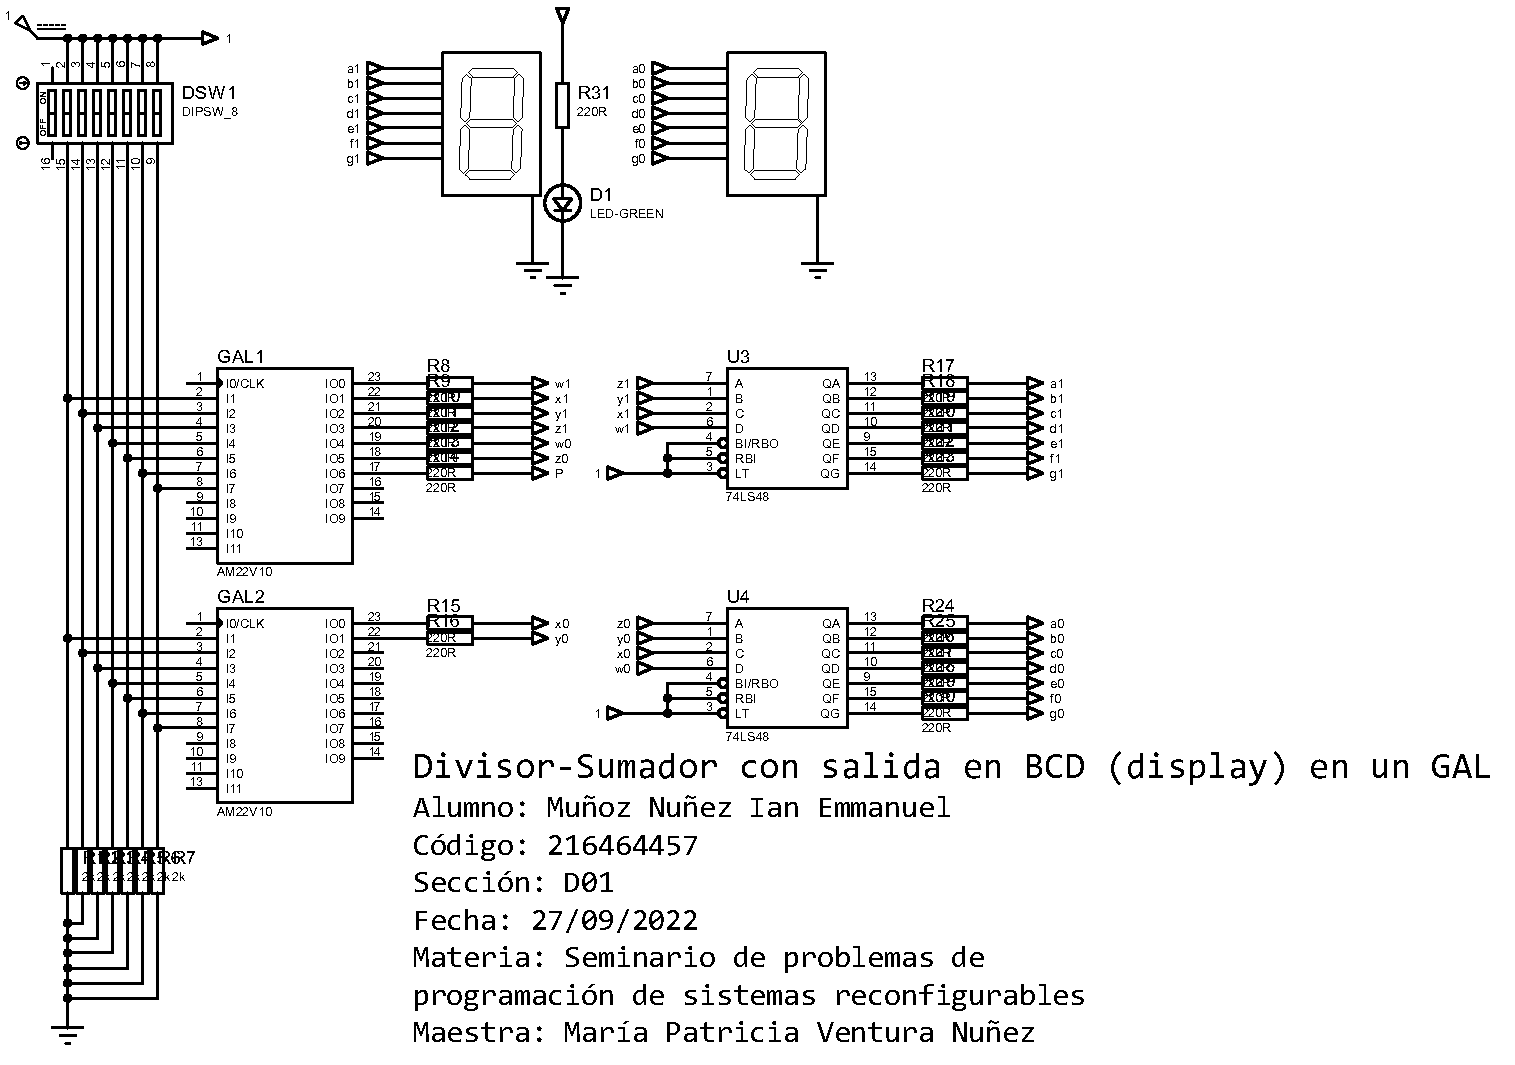
\includepdf[pages={1}]{main.PDF}
}

\newpage
\subsection{Protoboard}
\begin{figure}[h!]
    \centering
    
    \begin{subfigure}[tl]{0.45\textwidth}
        \centering
        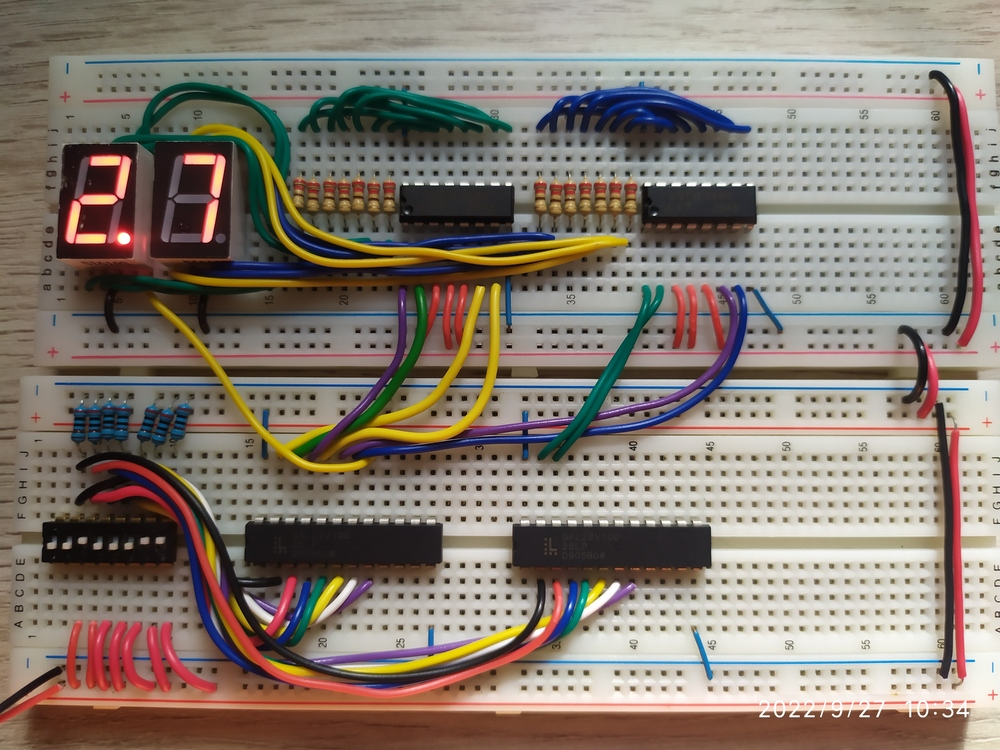
\includegraphics[width=\linewidth]{IMG_20220927_103402.jpg}
    \end{subfigure}
    \begin{subfigure}[tr]{0.45\textwidth}
        \centering
        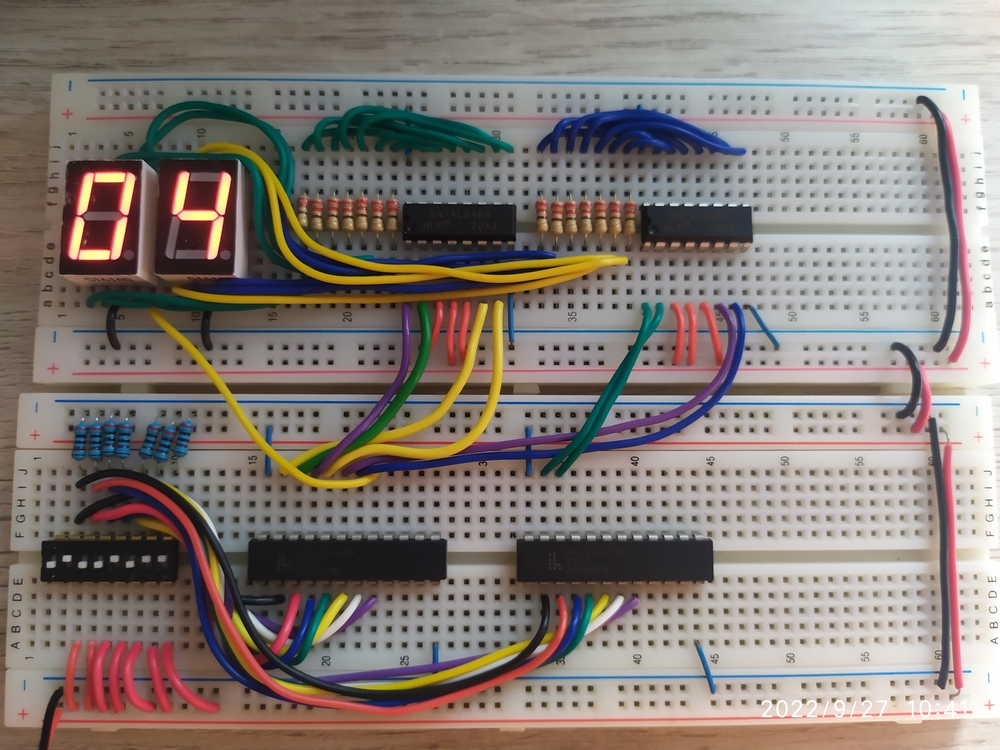
\includegraphics[width=\linewidth]{IMG_20220927_104146.jpg}
    \end{subfigure}
    \begin{subfigure}[bl]{0.45\textwidth}
        \centering
        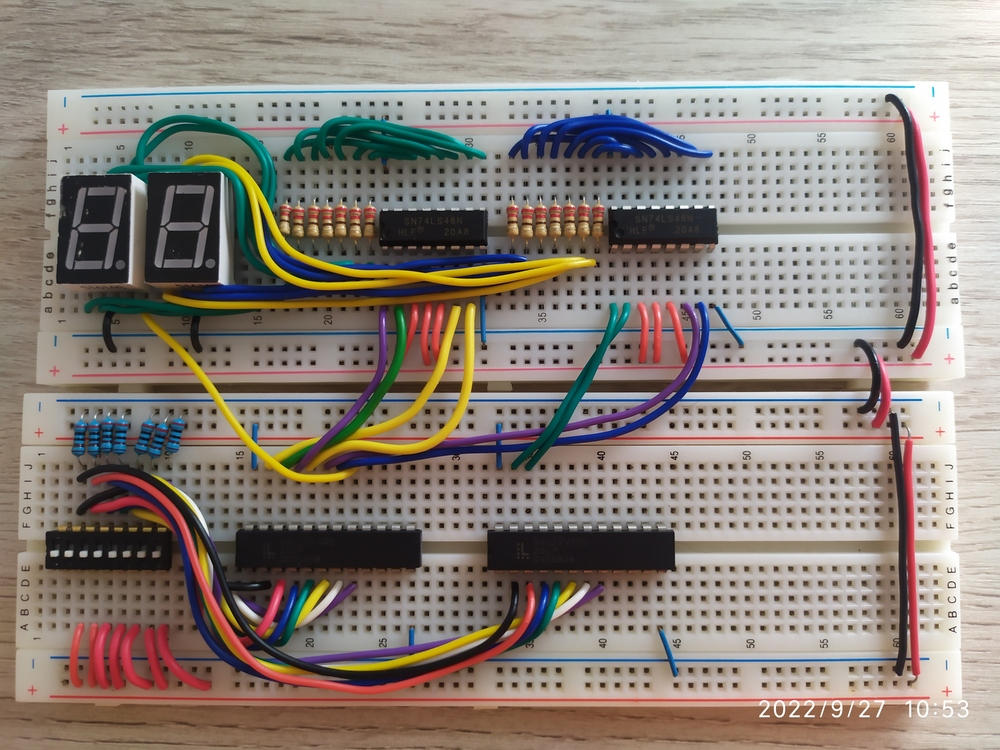
\includegraphics[width=\linewidth]{IMG_20220927_105309.jpg}
    \end{subfigure}
    \begin{subfigure}[br]{0.45\textwidth}
        \centering
        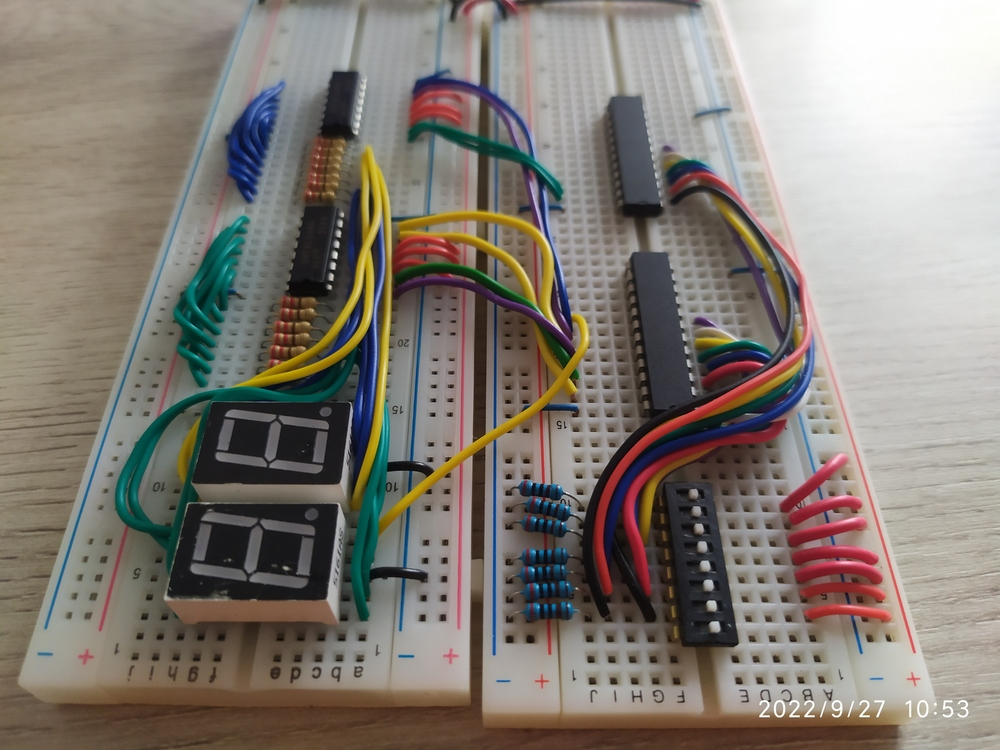
\includegraphics[width=\linewidth]{IMG_20220927_105322.jpg}
    \end{subfigure}
    
    \caption{\sffamily Circuito en protoboard}
    \label{fig:proto}
\end{figure}

\section{Conclusión}
{\sffamily\large
    \hspace{0.5cm} Este fue un proyecto extenso, tanto por las 128 combinaciones que se tenían que realizar como por los problemas que se tuvieron con las \emph{GAL}, pero al final el resultado me gusto mucho, ha sido de los proyectos que más me ha gustado hacer y de los que más problemas me ha dado.
}
    
\end{document}
